% ---------------------------------------------------------------------------
% To submit to PRD, replace the first line with
%   \documentclass[aps,prd,twocolumn,superscriptaddress,nofootinbib]{revtex4-2}
% and delete the \geometry / \title-block emulation below.
% ---------------------------------------------------------------------------
\documentclass[10pt,twocolumn]{article}
\usepackage[a4paper,margin=1.9cm,columnsep=0.7cm]{geometry}
\usepackage{amsmath,amssymb}
\usepackage{booktabs,multirow}
\usepackage{graphicx}
\usepackage[numbers,sort&compress]{natbib}
\usepackage[hidelinks]{hyperref}
\usepackage{xcolor}
\newcommand{\todo}[1]{\textcolor{red}{[#1]}}
\newenvironment{acknowledgments}{\section*{Acknowledgments}}{}
\newcommand{\Bc}{B_c}
\newcommand{\Bcs}{B_c^*}
\newcommand{\cc}{c\bar c}
\newcommand{\bb}{b\bar b}
\newcommand{\cb}{c\bar b}
\newcommand{\MeV}{\,\mathrm{MeV}}
\newcommand{\GeV}{\,\mathrm{GeV}}
\graphicspath{{figures/}}

\begin{document}

\twocolumn[
\begin{@twocolumnfalse}
\begin{center}
{\LARGE\bfseries How well do charmonium and bottomonium determine the $\Bc$ spectrum?}

\vspace{2pt}
{\large A potential-model test with the $\Bc(2S)$ hyperfine difference}

\vspace{10pt}
{\large Peter Agyemang Oppong}

\vspace{2pt}
{\small\itshape School of Physics and Astronomy, University of Glasgow, Glasgow G12 8QQ, United Kingdom}

\vspace{2pt}
{\small \today}
\end{center}
\begin{quote}\small
We ask to what extent the spectrum of the $\Bc$ meson is fixed by charmonium and bottomonium data alone.
Three families of spin-independent potentials---Cornell, logarithmic, and a power law with variable confining exponent $\alpha$---are refitted, together with the quark masses and the strong coupling, to 27 $J$-resolved $\cc$ and $\bb$ levels from the 2024 Review of Particle Physics, with spin-dependent splittings treated in first-order perturbation theory.
Without any $\Bc$ input the predictions for $\Bc(1S)$, $\Bcs(1S)$ and $\Bc(2S)$ agree across families to $\pm15\MeV$, while $P$-, $D$- and higher $S$-wave levels show $20$--$150\MeV$ model dependence that we quantify as a function of $\alpha$.
The $\cc+\bb$ data strongly favour a nearly logarithmic potential ($\alpha\lesssim0.1$).
The difference of hyperfine splittings $\Delta_{1S}-\Delta_{2S}$, which CMS and LHCb measure at $29$--$31\MeV$, is predicted at $28$--$40\MeV$ and independently selects $\alpha\simeq0.1$--$0.2$.
With a fixed $\alpha_s$ the absolute $1S$ hyperfine splitting comes out at $76$--$82\MeV$, well above the $64.5\pm1.7\MeV$ recently measured by ATLAS; a one-loop running coupling with $\Lambda$ determined by $\cc+\bb$ alone predicts $\Delta_{1S}=63$--$72\MeV$ and $\Delta_{2S}=34$--$38\MeV$, reproducing the ATLAS, CMS and LHCb hyperfine measurements simultaneously without any $\Bc$ input.
The spin-averaged $\Bc(2S)$ is predicted $11$--$24\MeV$ above the measured value in every variant.
We also give $E1$ and $M1$ radiative widths for the lowest excited $\Bc$ states.
\end{quote}
\vspace{6pt}
\end{@twocolumnfalse}
]

% ===========================================================================
\section{Introduction}
\label{sec:intro}

The $\Bc$ meson is the only hadron built from two heavy quarks of different flavour.
It is therefore both a laboratory for heavy-quark dynamics intermediate between charmonium and bottomonium and a stringent test of any description of the heavy quark--antiquark interaction: a model tuned on $\cc$ and $\bb$ must interpolate to $\cb$ with no additional freedom.
Experimentally the field has moved quickly.
The ground state is known to $0.3\MeV$~\cite{PDG2024}; CMS~\cite{CMS2019} and LHCb~\cite{LHCb2019} have observed the $\Bc(2S)$ and the $\Bcs(2S)$ doublet; lattice QCD predicted the $\Bcs(1S)$ mass to better than $10\MeV$~\cite{HPQCD2010}; and in 2026 ATLAS observed the $\Bcs(1S)\to\Bc\gamma$ transition directly, measuring the hyperfine splitting $m(\Bcs)-m(\Bc)=64.5\pm1.4\,^{+1.0}_{-1.4}\MeV$~\cite{ATLAS2026}.
Excited $P$- and $D$-wave states are within reach of LHCb Run~3.

Non-relativistic potential models~\cite{Eichten1994,Godfrey2004,Ebert2003} have long been used to predict the $\Bc$ spectrum.
Recent work has extended them to higher excitations and radiative decays~\cite{Mony2026,BcSpectro2026}, and has begun to quantify parameter uncertainties with Bayesian methods~\cite{Mony2026}.
A common feature of these studies, however, is that the model parameters are calibrated, at least in part, on the $\Bc$ states themselves.
This makes agreement with $\Bc(1S)$ and $\Bc(2S)$ partly circular and obscures the question we wish to address here:
\emph{given only the $\cc$ and $\bb$ spectra, how well is the $\Bc$ spectrum determined, and which of its features are independent of the unknown form of the confining potential?}

We answer this by refitting three potential families to the current $\cc$ and $\bb$ data and propagating the fits to $\cb$ without further adjustment (Secs.~\ref{sec:framework}--\ref{sec:bc}).
We then confront the hyperfine sector with three independent measurements: the ATLAS $1S$ splitting, and the $\Bc(2S)$--$\Bcs(2S)$ doublet of CMS and LHCb, which determines the \emph{difference} of the $1S$ and $2S$ splittings---a quantity in which the leading systematic uncertainties of the contact interaction cancel (Sec.~\ref{sec:hyperfine}).
Radiative widths are given in Sec.~\ref{sec:radiative} and we conclude in Sec.~\ref{sec:conclusions}.

% ===========================================================================
\section{Framework}
\label{sec:framework}

\subsection{Spin-independent spectrum}

For a quark of mass $m_1$ and antiquark of mass $m_2$ interacting through a central potential $V(r)$, the reduced radial wave function $u_{nl}(r)=rR_{nl}(r)$ obeys
\begin{equation}
  u'' = 2\mu\Big[V(r)+\frac{l(l+1)}{2\mu r^2}-E_{nl}\Big]u ,\qquad \mu=\frac{m_1m_2}{m_1+m_2},
  \label{eq:radial}
\end{equation}
in natural units.
We integrate Eq.~(\ref{eq:radial}) with the Numerov algorithm on a uniform grid ($h=10^{-3}\GeV^{-1}$) and locate eigenvalues by bisection on the number of radial nodes; the results are converged to better than $10^{-6}\GeV$ with respect to $h$ and the integration range.
The spin-averaged mass is $M_{nl}=m_1+m_2+E_{nl}$.

We consider three families of potential:
\begin{align}
  V_{\rm C}(r) &= -\frac{\kappa}{r}+\frac{r}{a^2}, \label{eq:cornell}\\
  V_{\rm L}(r) &= D + C\ln r, \label{eq:log}\\
  V_{\alpha}(r) &= V_0 + B\,(r^{\alpha}-1), \label{eq:power}
\end{align}
with $r$ in $\GeV^{-1}$.
Eq.~(\ref{eq:cornell}) is the Cornell potential~\cite{Eichten1978}; Eq.~(\ref{eq:log}) the Quigg--Rosner logarithmic potential~\cite{Quigg1977}; Eq.~(\ref{eq:power}) is the Martin power law~\cite{Martin1980} written so that the potential is pinned at $r=1\GeV^{-1}$ ($V_0=-1.166\GeV$) and the exponent $\alpha$ can be varied without shifting the potential by amounts that the quark masses would otherwise absorb.
For $\alpha=0.1$ it coincides with the Martin potential of Ref.~\cite{Eichten1994}; as $\alpha\to0$ it tends to Eq.~(\ref{eq:log}) with $C=B\alpha$; $\alpha=1$ is linear confinement.
The additive constants $D$ and $V_0$ are exactly degenerate with $m_1+m_2$ and are held fixed.

\subsection{Spin-dependent splittings}

Fine and hyperfine structure is added in first-order perturbation theory following Eichten and Quigg~\cite{Eichten1994},
\begin{equation}
  \Delta = \sum_{k=1}^4 T_k,
\end{equation}
\begin{align}
  T_1 &= \Big[\frac{\langle\mathbf L\!\cdot\!\mathbf s_1\rangle}{2m_1^2}+\frac{\langle\mathbf L\!\cdot\!\mathbf s_2\rangle}{2m_2^2}\Big]\tilde T_1,\quad
  T_2 = \frac{\langle\mathbf L\!\cdot\!\mathbf s_1\rangle+\langle\mathbf L\!\cdot\!\mathbf s_2\rangle}{m_1m_2}\tilde T_2,\notag\\
  T_3 &= \frac{\langle\mathbf s_1\!\cdot\!\mathbf s_2\rangle}{m_1m_2}\tilde T_3,\qquad
  T_4 = \frac{\langle S_{12}\rangle}{m_1m_2}\tilde T_4,
\end{align}
with radial coefficients
\begin{align}
  \tilde T_1 &= -\Big\langle\frac1r\frac{dV}{dr}\Big\rangle+2\tilde T_2, &
  \tilde T_2 &= \frac{4\alpha_s}{3}\langle r^{-3}\rangle,\notag\\
  \tilde T_3 &= \frac{8\alpha_s}{9}|R_{n0}(0)|^2, &
  \tilde T_4 &= \frac{\alpha_s}{3}\langle r^{-3}\rangle .
  \label{eq:Ttilde}
\end{align}
The full fitted potential is treated as a Lorentz scalar for the spin--orbit term, while the vector one-gluon exchange enters through $\alpha_s$; this is the prescription of Ref.~\cite{Eichten1994} and keeps the spin-dependent sector free of additional parameters.
For $m_1\neq m_2$ the states with $J=L$ mix; we construct the $2\times2$ matrix in the $\{{}^3L_L,{}^1L_L\}$ basis,
\begin{equation}
  H=\begin{pmatrix} -\tfrac12(a_1+a_2)+2d & \tfrac12(a_1-a_2)\sqrt{L(L+1)}\\ \tfrac12(a_1-a_2)\sqrt{L(L+1)} & 0\end{pmatrix},
\end{equation}
with $a_i=\tilde T_1/2m_i^2+\tilde T_2/m_1m_2$ and $d=\tilde T_4/m_1m_2$, and diagonalise it.
Its trace and determinant agree with the $jj$-coupling matrices of Ref.~\cite{Eichten1994}, Eqs.~(2.21).
We label the two $J=L$ eigenstates $L^{+}$ and $L^{+\prime}$ in order of mass.

Two treatments of $\alpha_s$ are compared.
In the \emph{fixed} variant $\alpha_s$ is a single fitted constant.
In the \emph{running} variant we use the one-loop expression $\alpha_s(\mu)=12\pi/[25\ln(\mu^2/\Lambda^2)]$ ($n_f=4$) evaluated at a scale set by the quark masses, either $\mu=2\mu_{\rm red}=2m_1m_2/(m_1+m_2)$ or $\mu=\sqrt{m_1m_2}$, and fit $\Lambda$ instead of $\alpha_s$.
The two scale choices coincide for $\cc$ and $\bb$ and differ only in how the coupling is interpolated to $\cb$.

\subsection{Radiative transitions}

$E1$ and $M1$ widths are computed from the same wave functions~\cite{Eichten1994},
\begin{align}
  \Gamma_{E1} &= \frac{4\alpha\langle e_Q\rangle^2}{27}\,k^3\,(2J_f+1)\,\mathcal S_{if}\,|\langle f|r|i\rangle|^2,\\
  \Gamma_{M1} &= \frac{16\alpha}{3}\,\mu_Q^2\,k^3\,(2J_f+1)\,|\langle f|j_0(kr/2)|i\rangle|^2,
\end{align}
with $\langle e_Q\rangle=(m_be_c-m_ce_{\bar b})/(m_b+m_c)$, $\mu_Q=(m_be_c-m_ce_{\bar b})/4m_cm_b$, $k=(M_i^2-M_f^2)/2M_i$, and $\mathcal S_{if}=9\max(L_i,L_f)\{^{L_f}_{J_i}\,^{J_f}_{L_i}\,^{S}_{1}\}^2$, which reduces to $\mathcal S=1$ for $^3S_1\leftrightarrow{}^3P_J$ and $\mathcal S=3$ for $^1P_1\leftrightarrow{}^1S_0$.
For spin-mixed states the $E1$ rate is the sum over the $S=1$ and $S=0$ channels weighted by the squared mixing amplitudes.
On charmonium this reproduces $\Gamma(\chi_{c0,1,2}\to J/\psi\gamma)=163,\,265,\,340\,$keV against the measured $151,\,288,\,374\,$keV~\cite{PDG2024}.

All code is public (see Code and data availability) and every table and figure in this paper is regenerated by a single script.

% ===========================================================================
\section{Fit to charmonium and bottomonium}
\label{sec:fit}

\begin{table}[t]
\caption{Experimental input: 27 $J$-resolved levels below open-flavour threshold~\cite{PDG2024}, in MeV. Our radial label $n$ counts excitations from 1, so $\chi_c(1P)$ is $1\,^3P_J$. $\Upsilon(4S)$ is excluded.}
\label{tab:data}
\centering\small
\begin{tabular}{llr}
\toprule
System & State & Mass \\
\midrule
$c\bar c$ & $1\,^1S_0$ & $2984.1 \pm 0.3$ \\
$c\bar c$ & $1\,^3S_1$ & $3096.9 \pm 0.0$ \\
$c\bar c$ & $1\,^3P_0$ & $3415.5 \pm 0.2$ \\
$c\bar c$ & $1\,^3P_1$ & $3510.7 \pm 0.1$ \\
$c\bar c$ & $1\,^1P_1$ & $3525.4 \pm 0.1$ \\
$c\bar c$ & $1\,^3P_2$ & $3556.2 \pm 0.1$ \\
$c\bar c$ & $2\,^1S_0$ & $3637.8 \pm 0.6$ \\
$c\bar c$ & $2\,^3S_1$ & $3686.1 \pm 0.0$ \\
$c\bar c$ & $1\,^3D_1$ & $3773.7 \pm 0.7$ \\
$c\bar c$ & $1\,^3D_2$ & $3823.5 \pm 0.3$ \\
$c\bar c$ & $1\,^3D_3$ & $3842.7 \pm 0.2$ \\
$b\bar b$ & $1\,^1S_0$ & $9398.7 \pm 2.0$ \\
$b\bar b$ & $1\,^3S_1$ & $9460.4 \pm 0.1$ \\
$b\bar b$ & $1\,^3P_0$ & $9859.4 \pm 0.5$ \\
$b\bar b$ & $1\,^3P_1$ & $9892.8 \pm 0.4$ \\
$b\bar b$ & $1\,^1P_1$ & $9899.3 \pm 0.8$ \\
$b\bar b$ & $1\,^3P_2$ & $9912.2 \pm 0.4$ \\
$b\bar b$ & $2\,^1S_0$ & $9999.0 \pm 3.5$ \\
$b\bar b$ & $2\,^3S_1$ & $10023.4 \pm 0.5$ \\
$b\bar b$ & $1\,^3D_2$ & $10163.7 \pm 1.4$ \\
$b\bar b$ & $2\,^3P_0$ & $10232.5 \pm 0.6$ \\
$b\bar b$ & $2\,^3P_1$ & $10255.5 \pm 0.6$ \\
$b\bar b$ & $2\,^1P_1$ & $10259.8 \pm 1.2$ \\
$b\bar b$ & $2\,^3P_2$ & $10268.6 \pm 0.6$ \\
$b\bar b$ & $3\,^3S_1$ & $10355.1 \pm 0.5$ \\
$b\bar b$ & $3\,^3P_1$ & $10513.4 \pm 0.7$ \\
$b\bar b$ & $3\,^3P_2$ & $10524.0 \pm 0.8$ \\
\bottomrule

\end{tabular}
\end{table}

\begin{table*}[t]
\caption{Fitted parameters and $\chi^2$ per degree of freedom for a $10\MeV$ theory floor. Units: $B$, $C$, $m_c$, $m_b$, $\Lambda$ in GeV; $a$ in GeV$^{-1}$. For the Martin family $B$, $m_c$ and $m_b$ are strongly correlated (see text); the individual errors are large but predicted masses are not.}
\label{tab:params}
\centering\small
\begin{tabular}{llp{11.5cm}}
\toprule
Family & $\chi^2$/dof & Parameters \\
\midrule
Martin & 84.7/22 & $B = 7.19 \pm 0.45$, $\alpha = 0.096(6)$, $m_c = 1.63 \pm 0.25$, $m_b = 5.02 \pm 0.23$, $\alpha_s = 0.457(26)$ \\
Log & 73.3/23 & $C = 0.737(5)$, $m_c = 1.509(4)$, $m_b = 4.908(2)$, $\alpha_s = 0.448(22)$ \\
Cornell & 133.7/22 & $\kappa = 0.456(10)$, $a = 2.328(20)$, $m_c = 1.334(9)$, $m_b = 4.752(7)$, $\alpha_s = 0.373(19)$ \\
Martin, running $\alpha_s$ & 69.8/22 & $B = 6.84 \pm 0.49$, $\alpha = 0.101(7)$, $m_c = 1.82 \pm 0.27$, $m_b = 5.20 \pm 0.26$, $\Lambda = 0.429(94)$ \\
Log, running $\alpha_s$ & 58.8/23 & $C = 0.740(5)$, $m_c = 1.509(4)$, $m_b = 4.905(2)$, $\Lambda = 0.332(25)$ \\
\bottomrule

\end{tabular}
\end{table*}

\begin{figure*}[t]
\centering
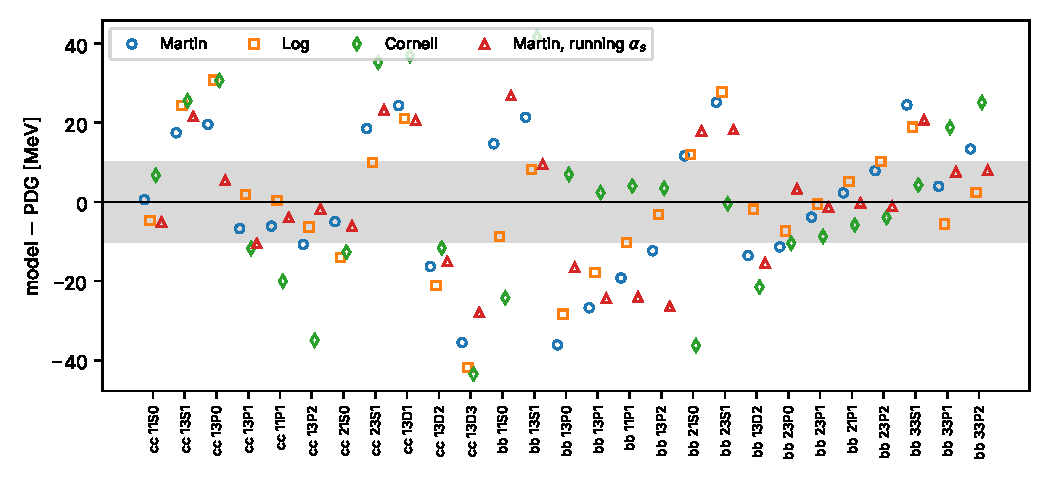
\includegraphics[width=\textwidth]{fig1_residuals}
\caption{Residuals (model $-$ PDG) of the fits for the three potential families and the running-coupling Martin fit. The grey band is the $10\MeV$ theory floor.}
\label{fig:residuals}
\end{figure*}

Table~\ref{tab:data} lists the input.
We fit each family's potential parameters, $m_c$, $m_b$ and $\alpha_s$ (or $\Lambda$) by least squares to all 27 levels, using $\sigma^2=\sigma_{\rm exp}^2+\sigma_{\rm th}^2$ with a theory floor $\sigma_{\rm th}=10\MeV$ so that the keV-precision $J/\psi$ and $\psi(2S)$ masses do not dominate a model whose intrinsic accuracy is tens of MeV.
Parameter uncertainties are taken from the covariance of the fit and later propagated linearly to predictions.

The results are in Table~\ref{tab:params} and Fig.~\ref{fig:residuals}.
Residuals are typically $10$--$30\MeV$ and are largest for the charmonium $D$ waves (all families miss $\psi_3(3842)$ by $\sim40\MeV$), which lie at the $D\bar D$ threshold where coupled-channel effects are expected.
Compared with the 1994 parameters~\cite{Eichten1994}, the logarithmic and Martin families change little except for $\alpha_s$, which rises from $0.37$--$0.43$ to $0.45$--$0.46$; the Cornell quark masses, by contrast, drop by $0.4$--$0.5\GeV$, confirming that the original Cornell masses were tuned to a different mass convention.
The running coupling improves the fit in both families it was applied to ($\chi^2$: $85\to70$ for Martin, $74\to59$ for logarithmic) because it allows the $\cc$ and $\bb$ hyperfine splittings, $113$ and $62\MeV$, to be reproduced simultaneously; the fitted $\Lambda=0.33$--$0.43\GeV$ corresponds to $\alpha_s(m_c)\simeq0.50$ and $\alpha_s(m_b)\simeq0.28$--$0.30$.

For the Martin family the parameters $B$, $m_c$ and $m_b$ carry large formal errors because $B(r^\alpha-1)\simeq B\alpha\ln r$ for small $\alpha$, so $B$ and the masses are nearly degenerate.
The combination $m_c+m_b$ that enters $\Bc$ is nevertheless well constrained, and the propagated uncertainties on predicted masses are $\lesssim15\MeV$.

\begin{figure}[t]
\centering
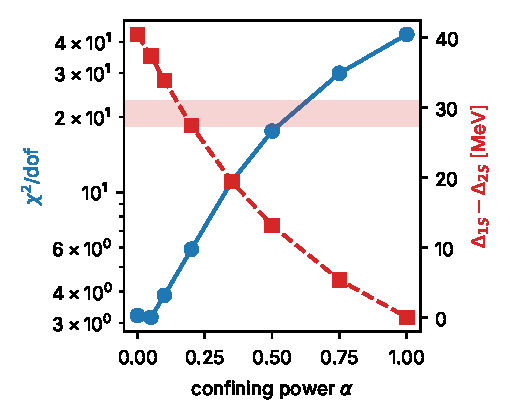
\includegraphics[width=\columnwidth]{fig2_chi2_alpha}
\caption{Left axis: $\chi^2$/dof of the $\cc+\bb$ fit as a function of the confining power $\alpha$ in Eq.~(\ref{eq:power}). Right axis: the predicted hyperfine difference $\Delta_{1S}-\Delta_{2S}$ of $\Bc$; the band is the CMS measurement~\cite{CMS2019}.}
\label{fig:chi2alpha}
\end{figure}

To probe the shape of the confining potential we repeat the fit of Eq.~(\ref{eq:power}) at fixed $\alpha\in\{0.05,0.1,0.2,0.35,0.5,0.75,1\}$ (Table~\ref{tab:scan}, Fig.~\ref{fig:chi2alpha}).
The $\chi^2$ rises monotonically from $73$ at $\alpha=0.05$ to $986$ at $\alpha=1$: the $\cc$ and $\bb$ spectra together strongly prefer a nearly logarithmic potential, consistent with the classic observation that the $2S$--$1S$ spacing is almost flavour independent~\cite{Quigg1977}.
A free fit of $\alpha$ returns $0.096(6)$.

\begin{table*}[t]
\caption{Fits at fixed confining power $\alpha$ and the resulting $\Bc$ levels (MeV). Centroids are spin-weighted averages of the fine-structure multiplets. The last column is the predicted $\Delta_{1S}-\Delta_{2S}$; experiment gives $29.1\pm1.7\MeV$~\cite{CMS2019}. $\alpha=0$ denotes the logarithmic fit.}
\label{tab:scan}
\centering\small
\begin{tabular}{lccccccccc}
\toprule
$\alpha$ & $\chi^2$/dof & $\alpha_s$ & $\Bc(1S)$ & $\Bcs(1S)$ & $\Bc(2S)$ & $1P$ & $1D$ & $3\,^3S_1$ & $\Delta_{1S}-\Delta_{2S}$ \\
\midrule
0 & 73/23 & 0.448 & 6266 & 6349 & 6889 & 6768 & 7043 & 7253 & 40.3 \\
0.05 & 72/23 & 0.461 & 6257 & 6337 & 6878 & 6752 & 7030 & 7254 & 37.2 \\
0.1 & 85/22 & 0.457 & 6267 & 6343 & 6886 & 6753 & 7034 & 7270 & 33.8 \\
0.2 & 136/23 & 0.465 & 6269 & 6338 & 6882 & 6737 & 7023 & 7285 & 27.3 \\
0.35 & 254/23 & 0.465 & 6280 & 6340 & 6886 & 6724 & 7014 & 7312 & 19.4 \\
0.5 & 404/23 & 0.462 & 6292 & 6344 & 6889 & 6713 & 7006 & 7336 & 13.1 \\
0.75 & 689/23 & 0.457 & 6309 & 6351 & 6893 & 6698 & 6990 & 7371 & 5.3 \\
1 & 986/23 & 0.451 & 6325 & 6360 & 6897 & 6686 & 6976 & 7400 & 0.0 \\
\bottomrule

\end{tabular}
\end{table*}

% ===========================================================================
\section{The $\Bc$ spectrum}
\label{sec:bc}

\begin{table*}[t]
\caption{$\Bc$ spectrum (MeV) predicted from the $\cc+\bb$ fits with fixed $\alpha_s$. Parenthesised errors are the propagated fit uncertainties; the model spread is half the range over the three families. The comparison columns are Eichten and Quigg (Buchm\"uller--Tye potential)~\cite{Eichten1994} and PDG 2024~\cite{PDG2024}. Our $1P$ and $1D$ correspond to the $2P$ and $3D$ of the principal-quantum-number labelling.}
\label{tab:bc}
\centering\small
\begin{tabular}{lcccccc}
\toprule
State & Martin & Log & Cornell & mean $\pm$ spread & EQ94 & PDG \\
\midrule
$1\,^1S_0$ & $6267(11)$ & $6266(4)$ & $6295(4)$ & $6276 \pm 14$ & 6264 & $6274.5 \pm 0.32$ \\
$1\,^3S_1$ & $6343(10)$ & $6349(4)$ & $6376(4)$ & $6356 \pm 17$ & 6337 & $6339.0 \pm 1.7$ \\
$1\,^3P_0$ & $6692(15)$ & $6711(4)$ & $6724(4)$ & $6709 \pm 16$ & 6700 & -- \\
$1^{+}$ & $6735(13)$ & $6753(3)$ & $6753(3)$ & $6747 \pm 9$ & 6730 & -- \\
$1^{+'}$ & $6756(10)$ & $6770(3)$ & $6759(2)$ & $6762 \pm 7$ & 6736 & -- \\
$1\,^3P_2$ & $6774(10)$ & $6787(3)$ & $6770(3)$ & $6777 \pm 9$ & 6747 & -- \\
$2\,^1S_0$ & $6886(11)$ & $6889(2)$ & $6877(3)$ & $6884 \pm 6$ & 6856 & $6871.2 \pm 1.0$ \\
$2\,^3S_1$ & $6928(10)$ & $6931(2)$ & $6930(3)$ & $6930 \pm 1$ & 6899 & -- \\
$1\,^3D_1$ & $7029(14)$ & $7040(3)$ & $7036(3)$ & $7035 \pm 5$ & 7012 & -- \\
$1D_{2}$ & $7029(9)$ & $7037(3)$ & $7022(3)$ & $7029 \pm 7$ & 7009 & -- \\
$1D_{2}'$ & $7040(14)$ & $7050(3)$ & $7044(3)$ & $7044 \pm 5$ & 7012 & -- \\
$1\,^3D_3$ & $7035(9)$ & $7043(3)$ & $7027(3)$ & $7035 \pm 8$ & 7005 & -- \\
$2\,^3P_0$ & $7101(13)$ & $7102(4)$ & $7148(5)$ & $7117 \pm 23$ & 7108 & -- \\
$1^{+}$ & $7132(12)$ & $7131(3)$ & $7176(4)$ & $7146 \pm 23$ & 7135 & -- \\
$1^{+'}$ & $7151(10)$ & $7147(3)$ & $7185(4)$ & $7161 \pm 19$ & 7142 & -- \\
$2\,^3P_2$ & $7164(10)$ & $7159(3)$ & $7196(4)$ & $7173 \pm 19$ & 7153 & -- \\
$3\,^1S_0$ & $7239(11)$ & $7225(4)$ & $7290(6)$ & $7251 \pm 32$ & 7244 & -- \\
$3\,^3S_1$ & $7270(10)$ & $7253(4)$ & $7335(6)$ & $7286 \pm 41$ & 7280 & -- \\
\bottomrule

\end{tabular}
\end{table*}

\begin{figure*}[t]
\centering
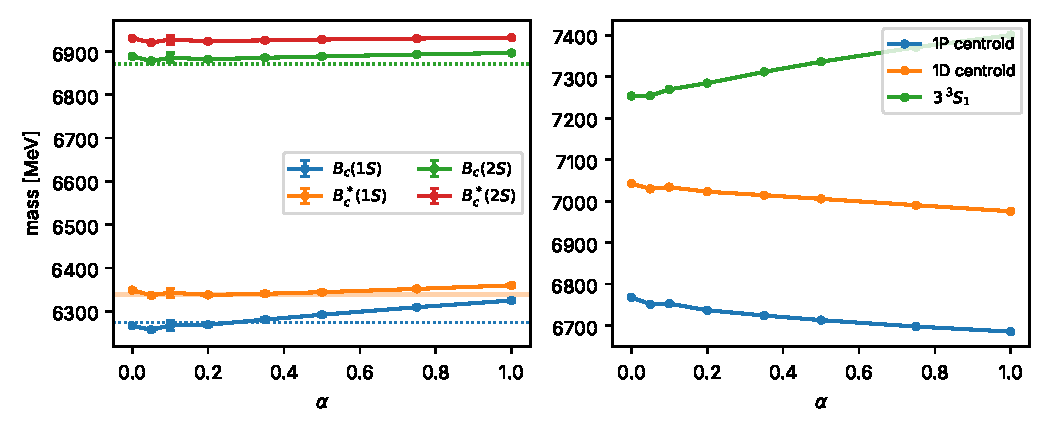
\includegraphics[width=\textwidth]{fig3_band}
\caption{$\Bc$ levels as a function of the confining power $\alpha$ of the potential fitted to $\cc+\bb$. Left: $S$-wave states; dotted lines are the measured $\Bc(1S)$ and $\Bc(2S)$, the band is the ATLAS $\Bcs(1S)$~\cite{ATLAS2026}. Right: $1P$ and $1D$ centroids and the $3\,^3S_1$.}
\label{fig:band}
\end{figure*}

Table~\ref{tab:bc} gives the $\Bc$ spectrum through $3S$, $2P$ and $1D$ predicted by the three families, and Fig.~\ref{fig:band} shows the dependence on $\alpha$ across the scan.
Three features stand out.

First, the $S$-wave levels are remarkably stable.
$\Bc(1S)$, $\Bcs(1S)$ and $\Bc(2S)$ vary by $\pm14$, $\pm17$ and $\pm6\MeV$ across the three families and by less than $70\MeV$ over the whole $\alpha$ scan, even though $\chi^2$ changes by an order of magnitude.
The ground state is reproduced at $6276\pm14\MeV$ against the measured $6274.5\MeV$ without any $\Bc$ input.

Second, the excited $P$, $D$ and $3S$ levels are not stable: the $1P$ centroid moves by $80\MeV$ and the $3\,^3S_1$ by $150\MeV$ between $\alpha=0$ and $\alpha=1$, and the Cornell family---which the $\cc+\bb$ fit disfavours---sits $30$--$60\MeV$ above the others for the $2P$ and $3S$.
These are the states for which future measurements will discriminate between confinement models; restricted to the $\alpha\lesssim0.2$ region preferred by $\cc+\bb$, the $1P$ centroid is $6737$--$6768\MeV$ and the $1D$ centroid $7023$--$7043\MeV$.

Third, the spin-averaged $\Bc(2S)$ is predicted $11$--$24\MeV$ \emph{above} the measured $6871.2\MeV$ in every one of the thirteen fits performed in this work (Tables~\ref{tab:bc} and \ref{tab:scan}), with a propagated uncertainty of only $2$--$11\MeV$.
Since the $\cc$ and $\bb$ $2S$ levels are themselves reproduced to $\lesssim25\MeV$ with residuals of both signs, this is a genuine interpolation failure at the few-MeV level rather than a fit artefact, and is the most robust discrepancy we find.
We return to it in Sec.~\ref{sec:conclusions}.

Our fixed-$\alpha_s$ $1P$ and $1D$ levels lie $5$--$30\MeV$ above those of Ref.~\cite{Eichten1994}, whose Buchm\"uller--Tye potential is softer at the relevant distances; the ordering within each multiplet and the mixing of the $J=L$ states (mixing angle $\simeq23^\circ$ for the $1P$) are the same.

% ===========================================================================
\section{The hyperfine test}
\label{sec:hyperfine}

\begin{table}[t]
\caption{Hyperfine splittings (MeV) of $\Bc$ predicted from $\cc+\bb$, for fixed and running $\alpha_s$. Experiment: $\Delta_{1S}=64.5\pm1.7$ and $M(\Bcs)=6339.0\pm1.7$ (ATLAS~\cite{ATLAS2026}); $\Delta_{1S}-\Delta_{2S}=29.1\pm1.7$ (CMS~\cite{CMS2019}) and $30.9$ (LHCb~\cite{LHCb2019}, statistical error $\approx1.5$); hence $\Delta_{2S}=35.4\pm2.4$. Lattice QCD (2010): $M(\Bcs)=6330\pm9$~\cite{HPQCD2010}.}
\label{tab:hyp}
\centering\small
\begin{tabular}{lcccc}
\toprule
Family & $\Delta_{1S}$ & $\Delta_{2S}$ & $\Delta_{1S}-\Delta_{2S}$ & $M(\Bcs)$ \\
\midrule
Martin & 75.9 & 42.1 & 33.8 & 6343 \\
Log & 82.5 & 42.1 & 40.4 & 6349 \\
Cornell & 81.2 & 53.1 & 28.2 & 6376 \\
Martin, running ($\sqrt{m_cm_b}$) & 62.9 & 35.1 & 27.9 & 6331 \\
Martin, running ($2\mu$) & 67.4 & 37.6 & 29.9 & 6332 \\
Log, running ($\sqrt{m_cm_b}$) & 66.5 & 33.9 & 32.6 & 6342 \\
Log, running ($2\mu$) & 72.1 & 36.8 & 35.3 & 6344 \\
\bottomrule

\end{tabular}
\end{table}

\begin{figure}[t]
\centering
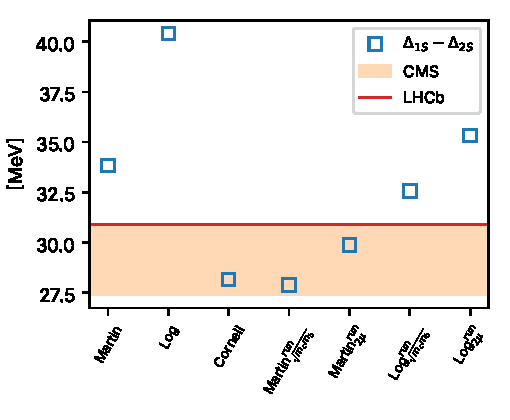
\includegraphics[width=\columnwidth]{fig4_hyperfine}
\caption{Predicted $\Delta_{1S}-\Delta_{2S}$ for each fit, compared with CMS (band) and LHCb (line).}
\label{fig:hyp}
\end{figure}

\begin{figure}[t]
\centering
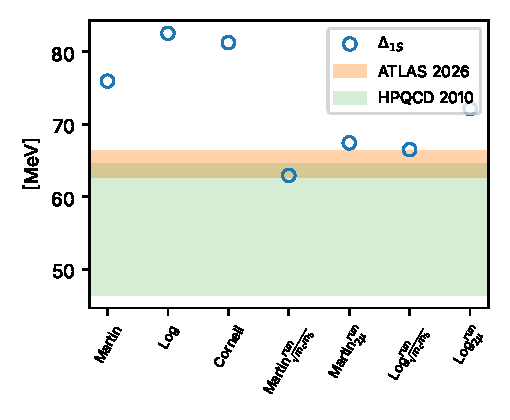
\includegraphics[width=\columnwidth]{fig5_hyperfine_abs}
\caption{Predicted absolute $1S$ hyperfine splitting $\Delta_{1S}$ for each fit, compared with the ATLAS measurement~\cite{ATLAS2026} (narrow band) and the 2010 lattice prediction~\cite{HPQCD2010} (wide band).}
\label{fig:hypabs}
\end{figure}

In both the CMS and LHCb analyses the $\Bcs(2S)$ is reconstructed through $\Bcs(2S)\to\Bcs(1S)\pi\pi$, $\Bcs(1S)\to\Bc\gamma$ with the soft photon unobserved, so the observed peak sits at $M(\Bcs(2S))-\Delta_{1S}$, where $\Delta_{nS}\equiv M(n^3S_1)-M(n^1S_0)$.
The measured separation of the two peaks is therefore
\begin{equation}
  M(\Bc(2S))-M_{\rm peak} = \Delta_{1S}-\Delta_{2S},
  \label{eq:observable}
\end{equation}
$=29.1\pm1.5\pm0.7\MeV$ (CMS~\cite{CMS2019}) and $30.9\MeV$ (LHCb~\cite{LHCb2019}).
This is a quantity in which potential models are unusually trustworthy.
From Eq.~(\ref{eq:Ttilde}),
\begin{equation}
  \Delta_{1S}-\Delta_{2S}=\frac{8\alpha_s}{9m_cm_b}\big[|R_{10}(0)|^2-|R_{20}(0)|^2\big],
\end{equation}
so the overall normalisation uncertainties of the contact interaction---the value of $\alpha_s$, relativistic corrections to $|R(0)|^2$, the choice of quark masses---enter as a common factor, while the shape of the potential enters through the ratio $|R_{20}(0)|^2/|R_{10}(0)|^2$.

Table~\ref{tab:hyp} and Fig.~\ref{fig:hyp} show that the three fixed-$\alpha_s$ families predict $\Delta_{1S}-\Delta_{2S}=28$--$40\MeV$, bracketing the measurement, and that across the $\alpha$ scan (Fig.~\ref{fig:chi2alpha}, Table~\ref{tab:scan}) the prediction falls smoothly from $37\MeV$ at $\alpha=0.05$ to zero at $\alpha=1$, where $|R_{n0}(0)|^2$ is independent of $n$.
The measurement therefore selects $\alpha\simeq0.1$--$0.2$, in agreement with---and independent of---the preference of the $\cc+\bb$ spectrum itself.
Two unrelated observables point to the same confining potential.

The absolute splitting is a sharper test still, now that ATLAS has measured it directly: $\Delta_{1S}=64.5\pm1.7\MeV$~\cite{ATLAS2026}, some $9\MeV$ (one standard deviation) above the 2010 lattice prediction~\cite{HPQCD2010}.
Combined with the CMS difference this fixes $\Delta_{2S}=35.4\pm2.4\MeV$, so the two lowest hyperfine splittings of $\Bc$ are both known to a few MeV.
Figure~\ref{fig:hypabs} and Table~\ref{tab:hyp} compare them with the predictions.
With fixed $\alpha_s$ all three families give $\Delta_{1S}=76$--$82\MeV$ and $\Delta_{2S}=42$--$53\MeV$, $10$--$20\MeV$ too high, even though each reproduces the $\cc$ and $\bb$ $1S$ splittings to $\lesssim20\MeV$: a single coupling cannot interpolate the contact term $\propto\alpha_s|R(0)|^2/m_1m_2$ between flavours.
With the one-loop running coupling the Martin family gives $\Delta_{1S}=63$--$67\MeV$, $\Delta_{2S}=35$--$38\MeV$ and $M(\Bcs)=6331$--$6332\MeV$, and the logarithmic family $\Delta_{1S}=67$--$72\MeV$, $\Delta_{2S}=34$--$37\MeV$---both within or close to the ATLAS and CMS uncertainties.
We stress that $\Lambda$ in these fits is determined by the $\cc$ and $\bb$ hyperfine splittings alone, and that neither a fixed coupling nor any adjustment of the spin-independent potential can reproduce the measured values.
A one-parameter running coupling fitted to equal-mass quarkonia therefore predicts the unequal-mass hyperfine sector of $\Bc$---the absolute $1S$ splitting, the $2S$ splitting and their difference---without $\Bc$ input.
The same fits place the lattice value~\cite{HPQCD2010} at the low edge of the allowed range; an updated lattice determination of $m(\Bcs)$ with current precision would be valuable.

% ===========================================================================
\section{Radiative transitions}
\label{sec:radiative}

\begin{table}[t]
\caption{$E1$ widths above $10\,$keV and $M1$ widths of the lowest $\Bc$ states, for the Martin fit with fixed $\alpha_s$. $k$ is the photon energy. Spin-mixed states are treated as described in Sec.~\ref{sec:framework}.}
\label{tab:rad}
\centering\small
\begin{tabular}{lccc}
\toprule
Transition & Type & $k$ [MeV] & $\Gamma$ [keV] \\
\midrule
$1^{+'}$ $\to$ $1\,^1S_0$$\,\gamma$ & E1 & 472 & 135.2 \\
$1\,^3P_2$ $\to$ $1\,^3S_1$$\,\gamma$ & E1 & 417 & 110.7 \\
$1\,^3D_1$ $\to$ $1\,^3P_0$$\,\gamma$ & E1 & 329 & 94.6 \\
$1\,^3D_3$ $\to$ $1\,^3P_2$$\,\gamma$ & E1 & 256 & 80.5 \\
$1^{+}$ $\to$ $1\,^3S_1$$\,\gamma$ & E1 & 381 & 71.2 \\
$1^{+'}$ $\to$ $2\,^1S_0$$\,\gamma$ & E1 & 260 & 65.6 \\
$1\,^3P_0$ $\to$ $1\,^3S_1$$\,\gamma$ & E1 & 340 & 59.9 \\
$2\,^3P_2$ $\to$ $2\,^3S_1$$\,\gamma$ & E1 & 232 & 57.1 \\
$1D_{2}'$ $\to$ $1^{+}$$\,\gamma$ & E1 & 298 & 52.5 \\
$1D_{2}$ $\to$ $1^{+'}$$\,\gamma$ & E1 & 267 & 46.6 \\
$1D_{2}'$ $\to$ $1^{+'}$$\,\gamma$ & E1 & 278 & 46.2 \\
$1D_{2}$ $\to$ $1^{+}$$\,\gamma$ & E1 & 287 & 42.4 \\
$1\,^3D_1$ $\to$ $1^{+}$$\,\gamma$ & E1 & 288 & 40.2 \\
$1^{+}$ $\to$ $2\,^3S_1$$\,\gamma$ & E1 & 201 & 30.4 \\
$2\,^3P_0$ $\to$ $2\,^3S_1$$\,\gamma$ & E1 & 172 & 23.0 \\
$1^{+}$ $\to$ $1\,^1S_0$$\,\gamma$ & E1 & 452 & 21.6 \\
$1^{+'}$ $\to$ $1\,^1S_0$$\,\gamma$ & E1 & 830 & 18.7 \\
$2\,^3P_2$ $\to$ $1\,^3S_1$$\,\gamma$ & E1 & 774 & 18.6 \\
$1^{+'}$ $\to$ $1\,^3S_1$$\,\gamma$ & E1 & 401 & 15.1 \\
$2\,^3S_1$ $\to$ $1\,^3P_2$$\,\gamma$ & E1 & 152 & 14.9 \\
$2\,^3P_0$ $\to$ $1\,^3S_1$$\,\gamma$ & E1 & 718 & 14.9 \\
$2\,^3S_1$ $\to$ $1^{+}$$\,\gamma$ & E1 & 190 & 14.7 \\
$2\,^1S_0$ $\to$ $1^{+'}$$\,\gamma$ & E1 & 128 & 13.6 \\
$1^{+}$ $\to$ $1\,^3S_1$$\,\gamma$ & E1 & 746 & 13.6 \\
$2\,^3P_2$ $\to$ $1\,^3D_3$$\,\gamma$ & E1 & 128 & 12.8 \\
$1^{+}$ $\to$ $2\,^1S_0$$\,\gamma$ & E1 & 242 & 11.9 \\
$1D_{2}'$ $\to$ $1\,^3P_2$$\,\gamma$ & E1 & 261 & 11.5 \\
$2\,^3S_1$ $\to$ $1\,^3P_0$$\,\gamma$ & E1 & 232 & 10.6 \\
$1\,^3S_1$ $\to$ $1\,^1S_0$$\,\gamma$ & M1 & 75 & 0.1 \\
$2\,^3S_1$ $\to$ $1\,^1S_0$$\,\gamma$ & M1 & 629 & 0.1 \\
$2\,^1S_0$ $\to$ $1\,^3S_1$$\,\gamma$ & M1 & 521 & 0.1 \\
$2\,^3S_1$ $\to$ $2\,^1S_0$$\,\gamma$ & M1 & 42 & 0.0 \\
\bottomrule

\end{tabular}
\end{table}

Table~\ref{tab:rad} lists the $E1$ and $M1$ widths of the $1P$, $1D$ and $2P$ states.
The $1P\to1S$ widths of $60$--$135\,$keV agree in magnitude with Refs.~\cite{Eichten1994,BcSpectro2026}; the spin mixing of the $1^+$ states redistributes the rate so that the heavier $1^{+\prime}$ decays mainly to $\Bc\gamma$ ($135\,$keV) and the lighter $1^+$ mainly to $\Bcs\gamma$ ($71\,$keV).
The $1D\to1P$ widths of $40$--$95\,$keV make the cascade $1D\to1P\gamma\to1S\gamma\gamma$ the natural route to the first $D$-wave $\Bc$ state.
The $M1$ rates are $\lesssim0.1\,$keV; the $\Bcs(1S)\to\Bc\gamma$ photon ($k\simeq60$--$75\MeV$) remains the principal obstacle to a direct $\Bcs$ mass measurement.
We have not included the model dependence of these widths, which is dominated by the photon energy ($\propto k^3$) and is therefore largest for transitions involving the excited levels of Sec.~\ref{sec:bc}.

% ===========================================================================
\section{Conclusions}
\label{sec:conclusions}

Fitting three families of potentials to the 2024 charmonium and bottomonium spectra and propagating them to $\cb$ without further input, we find:
\begin{enumerate}
\item The $\cc+\bb$ data prefer a nearly logarithmic confining potential, $\alpha\lesssim0.1$, and the $S$-wave $\Bc$ levels are determined to $\pm15\MeV$ independently of the potential; the $P$, $D$ and $3S$ levels are not, and are the states to measure.
\item The hyperfine difference $\Delta_{1S}-\Delta_{2S}$ measured by CMS and LHCb is predicted correctly from $\cc+\bb$ and independently selects $\alpha\simeq0.1$--$0.2$.
\item A fixed $\alpha_s$ overpredicts the $\Bcs(1S)$ hyperfine splitting measured by ATLAS by $10$--$20\MeV$; a one-loop running coupling, with $\Lambda$ fixed by $\cc$ and $\bb$, predicts $\Delta_{1S}=63$--$72\MeV$ and $\Delta_{2S}=34$--$38\MeV$, in agreement with ATLAS, CMS and LHCb simultaneously.
\item The spin-averaged $\Bc(2S)$ is predicted $11$--$24\MeV$ too high in every variant.
\end{enumerate}
The last point deserves comment.
The $2S$ discrepancy survives changes of confining potential, of $\alpha_s$ treatment and of theory floor, and is several times the propagated uncertainty.
It is the first level at which the first-order, non-relativistic treatment used here appears to fail for $\Bc$ while succeeding for $\cc$ and $\bb$, and we suggest that it reflects either relativistic corrections that do not interpolate linearly in $1/m$, or the proximity of the $2S$ to the $BD$ threshold.
A relativised treatment~\cite{Godfrey2004} or a coupled-channel calculation with the $\cc+\bb$-determined potential of this work would settle the question.

\begin{acknowledgments}
This work grew out of the author's MSc project in the School of Physics and Astronomy, University of Glasgow, supervised by Christine Davies, whose guidance on the potential-model treatment of heavy quarkonia is gratefully acknowledged.
The calculations are light enough to be reproduced in full on a single CPU core in under one hour; no high-performance computing resources were used.
An AI assistant (Claude, Anthropic) was used to refactor the thesis code into the package described here, to implement the spin-dependent, fitting and radiative-transition modules, and to help draft the manuscript; the author takes full responsibility for the physics, the code and the results.
\end{acknowledgments}

\section*{Code and data availability}
The complete code, the fitted parameter sets and the scripts that regenerate every table and figure in this paper are available at \url{https://github.com/apoppong24/bc-quarkonium}; the experimental inputs are listed in Table~\ref{tab:data}.

\bibliographystyle{unsrtnat}
\bibliography{refs}

\end{document}
